% Chapter 3, Topic _Linear Algebra_ Jim Hefferon
%  http://joshua.smcvt.edu/linearalgebra
%  2001-Jun-12
\topic{Rantai Markov}
\index{rantai Markov|(}

Berikut sebuah permainan sederhana:
seorang pemain bertaruh satu dolar pada setiap pelemparan koin,
dan permainan berakhir ketika uang pemain habis atau mencapai lima dolar.
Jika pemain mulai dengan tiga dolar, berapakah peluang permainan berlangsung
sekurang-kurangnya lima lemparan?
Dua puluh lima lemparan?

Pada setiap saat, pemain memiliki \$0, \$1, \ldots, atau \$5.
Kita mengatakan bahwa pemain berada dalam
\definend{keadaan}\index{keadaan}
$s_0$, $s_1$, \ldots, atau $s_5$.
Dalam permainan, pemain berpindah dari satu keadaan ke keadaan lain.
Sebagai contoh, pemain yang kini berada dalam keadaan $s_3$ memiliki peluang
$0.5$ untuk berpindah ke keadaan $s_2$ dan peluang $0.5$ untuk berpindah ke
$s_4$ pada lemparan berikutnya.
Keadaan batas berbeda; pemain tidak pernah meninggalkan keadaan~$s_0$ atau
keadaan~$s_5$.

Misalkan $p_{i}(n)$ adalah probabilitas bahwa pemain berada dalam keadaan
$s_{i}$ setelah $n$ lemparan.
Sebagai contoh, probabilitas berada dalam keadaan~$s_0$ setelah lemparan
ke-$n+1$ adalah
$p_{0}(n+1)=p_{0}(n)+0.5\cdot p_{1}(n)$.
Persamaan berikut merangkumnya.
\begin{equation*}
  % breqn didn't like this:
  % \begin{dmat}{D{.}{.}{1}D{.}{.}{1}D{.}{.}{1}D{.}{.}{1}D{.}{.}{1}D{.}{.}{1}}
    \begin{mat}
      1.0  &0.5  &0.0  &0.0  &0.0   &0.0  \\ 
      0.0  &0.0  &0.5  &0.0  &0.0   &0.0  \\ 
      0.0  &0.5  &0.0  &0.5  &0.0   &0.0  \\ 
      0.0  &0.0  &0.5  &0.0  &0.5   &0.0  \\ 
      0.0  &0.0  &0.0  &0.5  &0.0   &0.0  \\ 
      0.0  &0.0  &0.0  &0.0  &0.5   &1.0 
   \end{mat}  
   % \end{dmat}
   \colvec{p_{0}(n) \\ 
        p_{1}(n) \\
        p_{2}(n) \\
        p_{3}(n) \\
        p_{4}(n) \\
        p_{5}(n)}
   =\colvec{p_{0}(n+1) \\ 
        p_{1}(n+1) \\
        p_{2}(n+1) \\
        p_{3}(n+1) \\
        p_{4}(n+1) \\
        p_{5}(n+1)}
\end{equation*}

\textit{Sage} akan menghitung perkembangan permainan ini.
\begin{lstlisting}
sage: M = matrix(RDF, [[1.0, 0.0, 0.0, 0.0, 0.0, 0.0],
....:                  [0.5, 0.0, 0.5, 0.0, 0.0, 0.0],
....:                  [0.0, 0.5, 0.0, 0.5, 0.0, 0.0],
....:                  [0.0, 0.0, 0.5, 0.0, 0.5, 0.0],
....:                  [0.0, 0.0, 0.0, 0.5, 0.0, 0.5],
....:                  [0.0, 0.0, 0.0, 0.0, 0.0, 1.0]])
sage: M = M.transpose()
sage: v0 = vector(RDF, [0.0, 0.0, 0.0, 1.0, 0.0, 0.0])
sage: v1 = v0*M
sage: v1
(0.0, 0.0, 0.5, 0.0, 0.5, 0.0)
sage: v2 = v1*M
sage: v2
(0.0, 0.25, 0.0, 0.5, 0.0, 0.25)  
\end{lstlisting}
(Dua catatan: (1)~\textit{Sage} dapat menggunakan berbagai sistem bilangan
untuk membuat entri matriks; di sini kita menggunakan \textit{Real Double
Float}, dan (2)~\textit{Sage} lebih menyukai perkalian matriks dari kanan,
sebagai $\vec{v}\hspace{.1em}M$ alih-alih $M\vec{v}$ seperti yang biasa kita
gunakan, sehingga kita perlu mengambil transpos matriks.)

Berikut komponen-komponen vektor yang dihasilkan.
\begin{center}
  \begin{tabular}{@{}c|ccccc@{\hspace*{5em}}c@{}}
    $n=0$
    &\multicolumn{1}{c}{$n=1$}
    &\multicolumn{1}{c}{$n=2$}
    &\multicolumn{1}{c}{$n=3$}
    &\multicolumn{1}{c}{$n=4$}
    &\multicolumn{1}{c}{$\cdots$}
    &$n=24$ \\ 
    \hline  
    $\begin{array}{l}
             0 \\ 0    \\  0   \\  1    \\  0    \\  0
     \end{array}$
    % breqn again
    % &$\dcolvec[1]{
    %    0      \\  0    \\  0.5  \\  0    \\  0.5    \\  0
    %      }$
    % &$\dcolvec[2]{
    %   0      \\  .25  \\ 0    \\ .5    \\  0     \\  .25
    %      }$
    % &$\dcolvec[3]{
    %     .125   \\   0   \\ .375 \\ 0     \\ .25    \\  .25
    %       }$
    % &$\dcolvec[4]{
    %     .125   \\ .1875 \\ 0    \\ .3125 \\ 0      \\ .375
    %       }$
    % &$\cdots$
    % &$\dcolvec[5]{
    %     .39600 \\ .00276   \\ 0    \\ .00447 \\ 0  \\ .59676
    %       }$
    &$\begin{array}{l}
       0      \\  0    \\  0.5  \\  0    \\  0.5    \\  0
      \end{array}$
    &$\begin{array}{l}
      0      \\  0.25  \\ 0    \\ 0.5    \\  0     \\  0.25
      \end{array}$
    &$\begin{array}{l}
        0.125   \\   0   \\ 0.375 \\ 0     \\ 0.25    \\  0.25
       \end{array}$
    &$\begin{array}{l}
        0.125   \\ 0.187\,5 \\ 0    \\ 0.312\,5 \\ 0      \\ 0.375
       \end{array}$
    &  % $\cdots$
    &$\begin{array}{l}
        0.396\,00 \\ 0.002\,76   \\ 0    \\ 0.004\,47 \\ 0  \\ 0.596\,76
      \end{array}$
  \end{tabular}  
\end{center}
Permainan ini kecil kemungkinannya berlangsung lama karena pemain dengan cepat
berpindah ke keadaan akhir.
Sebagai contoh, setelah lemparan keempat sudah terdapat probabilitas $0.50$
bahwa permainan telah berakhir.
% (Because a player who enters either of the boundary states never leaves, they
% are said to be \definend{absorbtive}.)\index{state!absorbtive}

Ini merupakan \definend{rantai Markov}.\index{rantai Markov!definisi}
Setiap vektor merupakan
\definend{vektor probabilitas},\index{vektor!probabilitas}%
\index{vektor probabilitas} yang entri-entrinya berupa bilangan riil tak negatif
dan berjumlah $1$.
Matriks tersebut merupakan
\definend{matriks transisi}\index{matriks!transisi}%
\index{matriks transisi}
atau \definend{matriks stokastik},\index{matriks!stokastik}%
\index{matriks stokastik},
yang entri-entrinya berupa bilangan riil tak negatif dan setiap kolomnya
berjumlah $1$.

Salah satu ciri khas model rantai Markov adalah sifatnya yang
\definend{tanpa ingatan}\index{proses tanpa ingatan}%
\index{rantai Markov!tanpa ingatan}: keadaan berikutnya hanya bergantung pada
keadaan sekarang, bukan pada keadaan-keadaan sebelumnya.
Jadi, pemain yang tiba di $s_2$ dengan mulai dari keadaan $s_3$ lalu berpindah
ke keadaan~$s_2$ memiliki peluang yang tepat sama untuk selanjutnya berpindah
ke $s_3$ seperti pemain yang sebelumnya mulai di $s_3$, lalu berpindah ke
$s_4$, kemudian ke~$s_3$, dan akhirnya ke~$s_2$.

Berikut sebuah rantai Markov dari sosiologi.
Sebuah penelitian (\cite{MacdonaldRidge}, hlm.~202) membagi pekerjaan di
Britania Raya menjadi tiga tingkat: eksekutif dan tenaga profesional,
pengawas dan pekerja manual terampil, serta pekerja tidak terampil.
Para peneliti bertanya kepada sekitar dua ribu laki-laki, ``Pada tingkat mana
Anda berada, dan pada tingkat mana ayah Anda berada ketika Anda berusia empat
belas tahun?''
Di sini asumsi model Markov tentang riwayat mungkin tampak masuk akal\Dash kita
dapat menduga bahwa meskipun pekerjaan orang tua berpengaruh langsung terhadap
pekerjaan anak, pekerjaan kakek atau nenek kemungkinan tidak memiliki pengaruh
langsung semacam itu.
Berikut ringkasan kesimpulan penelitian tersebut.
\begin{equation*}
  % breqn again
  % \begin{dmat}{D{.}{.}{2}D{.}{.}{2}D{.}{.}{2}}
  \begin{mat}
    .60  &.29  &.16  \\
    .26  &.37  &.27  \\
    .14  &.34  &.57
  \end{mat}  
  % \end{dmat}
  \colvec{p_{U}(n) \\ p_{M}(n) \\ p_{L}(n)}
  =\colvec{p_{U}(n+1) \\ p_{M}(n+1) \\ p_{L}(n+1)}
\end{equation*} 
Sebagai contoh, jika kita meninjau kelas menengah pada generasi berikutnya,
anak seorang pekerja kelas atas memiliki probabilitas $0.26$ untuk menjadi
kelas menengah, anak seorang pekerja kelas menengah memiliki peluang $0.37$
untuk tetap berada di kelas menengah, dan anak seorang pekerja kelas bawah
memiliki probabilitas $0.27$ untuk menjadi kelas menengah.

\textit{Sage} akan menghitung tahap-tahap berturut-turut dari sistem ini
(distribusi kelas saat ini adalah $\vec{v}_0$).
\begin{lstlisting}
sage: M = matrix(RDF, [[0.60, 0.29, 0.16],
....:                  [0.26, 0.37, 0.27],
....:                  [0.14, 0.34, 0.57]])
sage: M = M.transpose()
sage: v0 = vector(RDF, [0.12, 0.32, 0.56])
sage: v0*M
(0.2544, 0.3008, 0.4448)
sage: v0*M^2
(0.31104, 0.297536, 0.391424)
sage: v0*M^3
(0.33553728, 0.2966432, 0.36781952)  
\end{lstlisting}
Berikut lima generasi selanjutnya.
Vektor-vektor ini memperlihatkan mobilitas ke atas, terutama pada generasi
pertama. Secara khusus, kelas bawah menyusut cukup banyak.
\begin{center}
  % breqn again
  \begin{tabular}{c|ccccc}
    $n=0$  &$n=1$  &$n=2$  &$n=3$  &$n=4$  &$n=5$  \\ \hline
    $\begin{array}{l}
               .12 \\ .32  \\ .56
      \end{array}$
    &$\begin{array}{l}
               .25 \\ .30  \\ .44
       \end{array}$
    &$\begin{array}{l}
               .31 \\ .30  \\ .39  
       \end{array}$
    &$\begin{array}{l}
               .34 \\ .30  \\ .37  
       \end{array}$
    &$\begin{array}{l}
               .35 \\ .30 \\ .36  
       \end{array}$
    &$\begin{array}{l}
               .35 \\ .30  \\ .35  
       \end{array}$
  \end{tabular}
\end{center}

Satu contoh lagi.
Dalam bisbol profesional Amerika terdapat dua liga, Liga Amerika dan Liga
Nasional. Pada akhir musim tahunan, tim pemenang Liga Amerika dan tim pemenang
Liga Nasional bertanding dalam Seri Dunia.
% what are these? (we follow [Brunner] but see also [Woodside]).
Pemenangnya adalah tim pertama yang meraih empat kemenangan.
Artinya, suatu seri berada dalam salah satu dari dua puluh empat keadaan:
$0$-$0$ (belum ada pertandingan yang dimenangi oleh kedua tim),
$1$-$0$ (satu kemenangan bagi tim Liga Amerika dan belum ada kemenangan bagi
tim Liga Nasional), dan seterusnya.

Tinjau suatu seri dengan probabilitas $p$ bahwa tim Liga Amerika memenangi
setiap pertandingan. Kita memperoleh hubungan berikut.
\begin{equation*}
  \begin{pmatrix}
    0      &0      &0      &0   &\ldots  \\
    p      &0      &0      &0   &\ldots  \\
    1-p    &0      &0      &0   &\ldots  \\
    0      &p      &0      &0   &\ldots  \\
    0      &1-p    &p      &0   &\ldots  \\
    0      &0      &1-p    &0   &\ldots  \\
    \vdots &\vdots &\vdots &\vdots
  \end{pmatrix}
  \colvec{p_{\text{0-0}}(n) \\ p_{\text{1-0}}(n) \\ p_{\text{0-1}}(n) \\
           p_{\text{2-0}}(n) \\ p_{\text{1-1}}(n) \\ p_{\text{0-2}}(n) \\ 
  \vdots }
  =
  \colvec{p_{\text{0-0}}(n+1) \\ p_{\text{1-0}}(n+1) \\ p_{\text{0-1}}(n+1) \\
           p_{\text{2-0}}(n+1) \\ p_{\text{1-1}}(n+1) \\ p_{\text{0-2}}(n+1) \\ 
           \vdots }
\end{equation*}
Kasus khusus yang sangat menarik terjadi ketika kedua tim berimbang,
$p=0.50$. Tabel di bawah mencantumkan komponen-komponen vektor yang dihasilkan
untuk $n=0$ hingga $n=7$.
% (The code to generate this table in the computer algebra system
% Octave follows the exercises.)

Perhatikan bahwa tim-tim yang berimbang cenderung menjalani seri yang
panjang\Dash terdapat probabilitas $0.625$ bahwa seri berlangsung sekurang-kurangnya
enam pertandingan.

\begin{center}\small
\newcommand{\markovspacer}{\hspace{.8em}}
\begin{tabular}{@{}r|c@{\markovspacer}c@{\markovspacer}c@{\markovspacer}c@{\markovspacer}c@{\markovspacer}c@{\markovspacer}c@{\markovspacer}c@{}}
      &$n=0$  &$n=1$  &$n=2$  &$n=3$  &$n=4$  &$n=5$  &$n=6$  &$n=7$  \\ \hline
  $\begin{array}{@{}c@{}}
    0-0 \\
    1-0 \\
    0-1 \\
    2-0 \\
    1-1 \\
    0-2 \\
    3-0 \\
    2-1 \\
    1-2 \\
    0-3 \\
    4-0 \\
    3-1 \\
    2-2 \\
    1-3 \\
    0-4 \\
    4-1 \\
    3-2 \\
    2-3 \\
    1-4 \\
    4-2 \\
    3-3 \\
    2-4 \\
    4-3 \\
    3-4 
  \end{array}$
  &$\begin{array}{l}
     1 \\
     0 \\
     0 \\
     0 \\
     0 \\
     0 \\
     0 \\
     0 \\
     0 \\
     0 \\
     0 \\
     0 \\
     0 \\
     0 \\
     0 \\
     0 \\
     0 \\
     0 \\
     0 \\
     0 \\
     0 \\
     0 \\
     0 \\
     0 
   \end{array}$
  &$\begin{array}{l}
        0           \\
        0.5         \\
        0.5         \\
        0           \\
        0           \\
        0           \\
        0           \\
        0           \\
        0           \\
        0           \\
        0           \\
        0           \\
        0           \\
        0           \\
        0           \\
        0           \\
        0           \\
        0           \\
        0           \\
        0           \\
        0           \\
        0           \\
        0           \\
        0              
   \end{array}$
  &$\begin{array}{l}
        0           \\
        0           \\
        0           \\
        0.25        \\
        0.5         \\
        0.25        \\
        0           \\
        0           \\
        0           \\
        0           \\
        0           \\
        0           \\
        0           \\
        0           \\
        0           \\
        0           \\
        0           \\
        0           \\
        0           \\
        0           \\
        0           \\
        0           \\
        0           \\
        0              
   \end{array}$
  &$\begin{array}{l}
        0            \\
        0            \\
        0            \\
        0            \\
        0            \\
        0            \\
        0.125        \\
        0.375        \\
        0.375        \\
        0.125        \\
        0            \\
        0            \\
        0            \\
        0            \\
        0            \\
        0            \\
        0            \\
        0            \\
        0            \\
        0            \\
        0            \\
        0            \\
        0            \\
        0              
   \end{array}$
  &$\begin{array}{l}
        0              \\
        0              \\
        0              \\
        0              \\
        0              \\
        0              \\
        0              \\
        0              \\
        0              \\
        0              \\
        0.062\,5         \\
        0.25           \\
        0.375          \\
        0.25           \\
        0.062\,5         \\
        0              \\
        0              \\
        0              \\
        0              \\
        0              \\
        0              \\
        0              \\
        0              \\
        0                      
   \end{array}$
  &$\begin{array}{l}
        0              \\
        0              \\
        0              \\
        0              \\
        0              \\
        0              \\
        0              \\
        0              \\
        0              \\
        0              \\
        0.062\,5         \\
        0              \\
        0              \\
        0              \\
        0.062\,5         \\
        0.125          \\
        0.312\,5         \\
        0.312\,5         \\
        0.125          \\
        0              \\
        0              \\
        0              \\
        0              \\
        0                      
   \end{array}$
  &$\begin{array}{l}
        0               \\
        0               \\
        0               \\
        0               \\
        0               \\
        0               \\
        0               \\
        0               \\
        0               \\
        0               \\
        0.062\,5          \\
        0               \\
        0               \\
        0               \\
        0.062\,5          \\
        0.125           \\
        0               \\
        0               \\
        0.125           \\
        0.156\,25         \\
        0.312\,5          \\
        0.156\,25         \\
        0               \\
        0                      
   \end{array}$
  &$\begin{array}{l}
        0             \\
        0             \\
        0             \\
        0             \\
        0             \\
        0             \\
        0             \\
        0             \\
        0             \\
        0             \\
        0.062\,5        \\
        0             \\
        0             \\
        0             \\
        0.062\,5        \\
        0.125         \\
        0             \\
        0             \\
        0.125         \\
        0.156\,25       \\
        0             \\
        0.156\,25       \\
        0.156\,25       \\
        0.156\,25        
   \end{array}$
  % f-ing breqn
  % &$\begin{aligncolondecimal}{0}
  %    1 \\
  %    0 \\
  %    0 \\
  %    0 \\
  %    0 \\
  %    0 \\
  %    0 \\
  %    0 \\
  %    0 \\
  %    0 \\
  %    0 \\
  %    0 \\
  %    0 \\
  %    0 \\
  %    0 \\
  %    0 \\
  %    0 \\
  %    0 \\
  %    0 \\
  %    0 \\
  %    0 \\
  %    0 \\
  %    0 \\
  %    0 
  %  \end{aligncolondecimal}$
  % &$\begin{aligncolondecimal}{1}
  %       0           \\
  %       0.5         \\
  %       0.5         \\
  %       0           \\
  %       0           \\
  %       0           \\
  %       0           \\
  %       0           \\
  %       0           \\
  %       0           \\
  %       0           \\
  %       0           \\
  %       0           \\
  %       0           \\
  %       0           \\
  %       0           \\
  %       0           \\
  %       0           \\
  %       0           \\
  %       0           \\
  %       0           \\
  %       0           \\
  %       0           \\
  %       0              
  %  \end{aligncolondecimal}$
  % &$\begin{aligncolondecimal}{2}
  %       0           \\
  %       0           \\
  %       0           \\
  %       0.25        \\
  %       0.5         \\
  %       0.25        \\
  %       0           \\
  %       0           \\
  %       0           \\
  %       0           \\
  %       0           \\
  %       0           \\
  %       0           \\
  %       0           \\
  %       0           \\
  %       0           \\
  %       0           \\
  %       0           \\
  %       0           \\
  %       0           \\
  %       0           \\
  %       0           \\
  %       0           \\
  %       0              
  %  \end{aligncolondecimal}$
  % &$\begin{aligncolondecimal}{3}
  %       0            \\
  %       0            \\
  %       0            \\
  %       0            \\
  %       0            \\
  %       0            \\
  %       0.125        \\
  %       0.375        \\
  %       0.375        \\
  %       0.125        \\
  %       0            \\
  %       0            \\
  %       0            \\
  %       0            \\
  %       0            \\
  %       0            \\
  %       0            \\
  %       0            \\
  %       0            \\
  %       0            \\
  %       0            \\
  %       0            \\
  %       0            \\
  %       0              
  %  \end{aligncolondecimal}$
  % &$\begin{aligncolondecimal}{4}
  %       0              \\
  %       0              \\
  %       0              \\
  %       0              \\
  %       0              \\
  %       0              \\
  %       0              \\
  %       0              \\
  %       0              \\
  %       0              \\
  %       0.0625         \\
  %       0.25           \\
  %       0.375          \\
  %       0.25           \\
  %       0.0625         \\
  %       0              \\
  %       0              \\
  %       0              \\
  %       0              \\
  %       0              \\
  %       0              \\
  %       0              \\
  %       0              \\
  %       0                      
  %  \end{aligncolondecimal}$
  % &$\begin{aligncolondecimal}{4}
  %       0              \\
  %       0              \\
  %       0              \\
  %       0              \\
  %       0              \\
  %       0              \\
  %       0              \\
  %       0              \\
  %       0              \\
  %       0              \\
  %       0.0625         \\
  %       0              \\
  %       0              \\
  %       0              \\
  %       0.0625         \\
  %       0.125          \\
  %       0.3125         \\
  %       0.3125         \\
  %       0.125          \\
  %       0              \\
  %       0              \\
  %       0              \\
  %       0              \\
  %       0                      
  %  \end{aligncolondecimal}$
  % &$\begin{aligncolondecimal}{5}
  %       0               \\
  %       0               \\
  %       0               \\
  %       0               \\
  %       0               \\
  %       0               \\
  %       0               \\
  %       0               \\
  %       0               \\
  %       0               \\
  %       0.0625          \\
  %       0               \\
  %       0               \\
  %       0               \\
  %       0.0625          \\
  %       0.125           \\
  %       0               \\
  %       0               \\
  %       0.125           \\
  %       0.15625         \\
  %       0.3125          \\
  %       0.15625         \\
  %       0               \\
  %       0                      
  %  \end{aligncolondecimal}$
  % &$\begin{aligncolondecimal}{5}
  %       0             \\
  %       0             \\
  %       0             \\
  %       0             \\
  %       0             \\
  %       0             \\
  %       0             \\
  %       0             \\
  %       0             \\
  %       0             \\
  %       0.0625        \\
  %       0             \\
  %       0             \\
  %       0             \\
  %       0.0625        \\
  %       0.125         \\
  %       0             \\
  %       0             \\
  %       0.125         \\
  %       0.15625       \\
  %       0             \\
  %       0.15625       \\
  %       0.15625       \\
  %       0.15625        
  %  \end{aligncolondecimal}$
\end{tabular}
\end{center}

Rantai Markov merupakan penerapan operasi matriks yang digunakan secara luas.
Rantai ini juga memberi kita contoh penggunaan matriks tanpa meninjau makna
pemetaan yang direpresentasikan oleh matriks tersebut.
Untuk pembahasan lebih lanjut tentang rantai Markov, tersedia banyak sumber,
antara lain \cite{KemenySnell} dan \cite{Iosifescu}.

\begin{exercises}
  % \item[]\textit{Use a computer for these problems.
  %   You can, for instance, adapt the Octave script given below.}
  \item 
    Pertanyaan-pertanyaan berikut merujuk pada permainan pelemparan koin.
    \begin{exparts}
     \partsitem Periksa perhitungan dalam tabel di akhir bagian pertama.
     \partsitem Tinjau baris kedua tabel vektor.
       Perhatikan bahwa baris ini memiliki nilai $0$ secara berselang-seling.
       Haruskah $p_{1}(j)$ bernilai $0$ ketika $j$ ganjil?
       Buktikan bahwa hal itu harus terjadi, atau berikan contoh penyangkal.
     \partsitem Lakukan eksperimen komputasi untuk memperkirakan peluang pemain
       mengakhiri permainan dengan lima dolar ketika mulai dengan satu dolar,
       dua dolar, dan empat dolar.
    \end{exparts}
    \begin{answer}
      \begin{exparts}
        \partsitem Dengan berkas \texttt{coin.m} berikut
\begin{computercode}         
# Fungsi Octave untuk permainan koin Markov. p adalah peluang turun.
function w = coin(p,v)
  q = 1-p;
  A=[1,p,0,0,0,0;
     0,0,p,0,0,0;
     0,q,0,p,0,0;
     0,0,q,0,p,0;
     0,0,0,q,0,0;
     0,0,0,0,q,1];
  w = A * v;
endfunction
\end{computercode}
         sesi Octave berikut menghasilkan keluaran yang ditampilkan.
\begin{computercode}
octave:1> v0=[0;0;0;1;0;0]
v0 =
  0
  0
  0
  1
  0
  0
octave:2> p=.5
p = 0.50000
octave:3> v1=coin(p,v0)
v1 =
  0.00000
  0.00000
  0.50000
  0.00000
  0.50000
  0.00000
octave:4> v2=coin(p,v1)
v2 =
  0.00000
  0.25000
  0.00000
  0.50000
  0.00000
  0.25000
\end{computercode}
Proses ini berlanjut terlalu banyak langkah untuk dicantumkan seluruhnya di sini.
\begin{computercode}
octave:26> v24=coin(p,v23)
v24 =
  0.39600
  0.00276
  0.00000
  0.00447
  0.00000
  0.59676
\end{computercode}        
        \partsitem Dengan menggunakan rumus-rumus berikut
          \begin{alignat*}{2}
             p_{1}(n+1) &= 0.5\cdot p_{2}(n)
             &\qquad
             p_{2}(n+1) &= 0.5\cdot p_{1}(n)+0.5\cdot p_{3}(n)
                                                              \\
             p_{3}(n+1) &= 0.5\cdot p_{2}(n)+0.5\cdot p_{4}(n)
             &\qquad
             p_{4}(n+1) &= 0.5\cdot p_{3}(n)             
          \end{alignat*}
          dan syarat awal berikut,
          \begin{equation*}
            \colvec{p_{0}(0) \\ p_{1}(0) \\ p_{2}(0) \\ p_{3}(0) \\ 
                        p_{4}(0) \\ p_{5}(0)}
            =
            \colvec{0 \\ 0 \\ 0 \\ 1 \\ 
                        0 \\ 0}
          \end{equation*} 
          kita akan membuktikan dengan induksi bahwa jika $n$ ganjil, maka
          $p_{1}(n)=p_{3}(n)=0$, dan jika $n$ genap, maka
          $p_{2}(n)=p_{4}(n)=0$.
          Pertama, berdasarkan syarat awal, pernyataan ini benar untuk kasus
          dasar $n=0$.
          Untuk langkah induksi, andaikan pernyataan benar bagi kasus
          $n=0$, $n=1$, \ldots, $n=k$, lalu tinjau kasus $n=k+1$.
          Jika $k+1$ ganjil, kedua persamaan
          \begin{align*}
             p_{1}(k+1) &= 0.5\cdot p_{2}(k)=0.5\cdot 0=0
                                                          \\
             p_{3}(k+1) &=0.5\cdot p_{2}(k)+0.5\cdot p_{4}(k)
                        =0.5\cdot 0+0.5\cdot 0
                        =0
          \end{align*}
          mengikuti hipotesis induksi $p_{2}(k)=p_{4}(k)=0$ karena $k$ genap.
          Kasus ketika $k+1$ genap serupa.
        \partsitem Kita dapat menggunakan, misalnya, $n=100$.
          Sesi Octave berikut
\begin{computercode}
octave:1> B=[1,.5,0,0,0,0;
>             0,0,.5,0,0,0;
>             0,.5,0,.5,0,0;
>             0,0,.5,0,.5,0;
>             0,0,0,.5,0,0;
>             0,0,0,0,.5,1];
octave:2> B100=B**100
B100 =
  1.00000  0.80000  0.60000  0.40000  0.20000  0.00000
  0.00000  0.00000  0.00000  0.00000  0.00000  0.00000
  0.00000  0.00000  0.00000  0.00000  0.00000  0.00000
  0.00000  0.00000  0.00000  0.00000  0.00000  0.00000
  0.00000  0.00000  0.00000  0.00000  0.00000  0.00000
  0.00000  0.20000  0.40000  0.60000  0.80000  1.00000
octave:3> B100*[0;1;0;0;0;0]
octave:4> B100*[0;0;1;0;0;0]
octave:5> B100*[0;0;0;1;0;0]
octave:6> B100*[0;0;0;0;1;0]
\end{computercode}
        menghasilkan keluaran berikut.
        \begin{equation*}
          \begin{array}{r|*{4}{c}}
            \multicolumn{1}{r}{\textit{mulai dengan:}}
            &\text{\$1}  &\text{\$2}  &\text{\$3}  &\text{\$4} \\ 
             \hline
               \begin{array}{c}
                 p_{0}(100) \\
                 p_{1}(100) \\
                 p_{2}(100) \\
                 p_{3}(100) \\
                 p_{4}(100) \\
                 p_{5}(100)
               \end{array}
               &\begin{aligncolondecimal}{5}
                 0.80000 \\
                 0.00000 \\
                 0.00000 \\
                 0.00000 \\
                 0.00000 \\
                 0.20000
               \end{aligncolondecimal}
               &\begin{aligncolondecimal}{5}
                    0.60000 \\
                    0.00000 \\
                    0.00000 \\
                    0.00000 \\
                    0.00000 \\
                    0.40000         
               \end{aligncolondecimal}
               &\begin{aligncolondecimal}{5}
                      0.40000 \\
                      0.00000 \\
                      0.00000 \\
                      0.00000 \\
                      0.00000 \\
                      0.60000           
               \end{aligncolondecimal}
               &\begin{aligncolondecimal}{5}
                   0.20000 \\
                   0.00000 \\
                   0.00000 \\
                   0.00000 \\
                   0.00000 \\
                   0.80000        
               \end{aligncolondecimal}
          \end{array}
        \end{equation*}
      \end{exparts}
    \end{answer}
  \item 
    \cite{Feller} % , p.~424.
    Kita meninjau pelemparan sebuah dadu dan mengatakan bahwa sistem berada
    dalam keadaan $s_i$ jika angka terbesar yang sejauh ini muncul pada dadu
    adalah $i$.
    Tuliskan $p_i(n)$ untuk probabilitas bahwa sistem berada dalam keadaan
    $s_i$ setelah $n$ lemparan.
    \begin{exparts}
      \partsitem Berikan matriks transisinya.
      \partsitem Mulai sistem dalam keadaan $s_1$, lalu jalankan selama lima
        lemparan. Apa vektor akhirnya?
    \end{exparts}
    \begin{answer}
      \begin{exparts}
        \partsitem Dari persamaan-persamaan berikut,
          \begin{equation*}
            \begin{linsys}{6}
              p_{1}(n)/6 &+ &0p_{2}(n) &+ &0p_{3}(n) 
                  &+ &0p_{4}(n) &+ &0p_{5}(n)  &+ &0p_{6}(n)  &= &p_{1}(n+1) \\
              p_{1}(n)/6 &+ &2p_{2}(n)/6 &+ &0p_{3}(n) 
                  &+ &0p_{4}(n) &+ &0p_{5}(n)  &+ &0p_{6}(n)  &= &p_{2}(n+1) \\
              p_{1}(n)/6 &+ &p_{2}(n)/6 &+ &3p_{3}(n)/6 
                  &+ &0p_{4}(n) &+ &0p_{5}(n)  &+ &0p_{6}(n)  &= &p_{3}(n+1) \\
              p_{1}(n)/6 &+ &p_{2}(n)/6 &+ &p_{3}(n)/6 
                  &+ &4p_{4}(n)/6 &+ &0p_{5}(n)  &+ &0p_{6}(n)  
                  &=  &p_{4}(n+1) \\
              p_{1}(n)/6 &+ &p_{2}(n)/6 &+ &p_{3}(n)/6 
                  &+ &p_{4}(n)/6 &+ &5p_{5}(n)/6  &+ &0p_{6}(n)  
                  &=  &p_{5}(n+1) \\
              p_{1}(n)/6 &+ &p_{2}(n)/6 &+ &p_{3}(n)/6 
                  &+ &p_{4}(n)/6 &+ &p_{5}(n)/6  &+ &6p_{6}(n)/6  
                  &=  &p_{6}(n+1) 
            \end{linsys}
          \end{equation*}
          kita memperoleh matriks transisi berikut.
          \begin{equation*}
            \begin{mat}
              1/6  &0   &0   &0   &0   &0  \\
              1/6  &2/6 &0   &0   &0   &0  \\
              1/6  &1/6 &3/6 &0   &0   &0  \\
              1/6  &1/6 &1/6 &4/6 &0   &0  \\
              1/6  &1/6 &1/6 &1/6 &5/6 &0  \\
              1/6  &1/6 &1/6 &1/6 &1/6 &6/6  
            \end{mat}
          \end{equation*}
       \partsitem Berikut sesi Octave, dengan keluarannya dihapus dan diringkas
         dalam tabel di bagian akhir.
\begin{computercode}
octave:1>   F=[1/6,  0,   0,   0,   0,   0;
>      1/6,  2/6, 0,   0,   0,   0; 
>      1/6,  1/6, 3/6, 0,   0,   0;  
>      1/6,  1/6, 1/6, 4/6, 0,   0; 
>      1/6,  1/6, 1/6, 1/6, 5/6, 0; 
>      1/6,  1/6, 1/6, 1/6, 1/6, 6/6];
octave:2> v0=[1;0;0;0;0;0]
octave:3> v1=F*v0
octave:4> v2=F*v1
octave:5> v3=F*v2
octave:6> v4=F*v3
octave:7> v5=F*v4
\end{computercode}
        Berikut hasilnya.
        \begin{equation*}
          \begin{array}{c|*{5}{c}}
            \multicolumn{1}{c}{\ }
            &1  &2  &3  &4 &5  \\ 
            \hline
               \begin{aligncolondecimal}{0}
                   1 \\
                   0 \\
                   0 \\
                   0 \\
                   0 \\
                   0              
               \end{aligncolondecimal}
               &\begin{aligncolondecimal}{5}
                    0.16667 \\
                    0.16667 \\
                    0.16667 \\
                    0.16667 \\
                    0.16667 \\
                    0.16667         
               \end{aligncolondecimal}
               &\begin{aligncolondecimal}{6}
                   0.027778 \\
                   0.083333 \\
                   0.138889 \\
                   0.194444 \\
                   0.250000 \\
                   0.305556       
               \end{aligncolondecimal}
               &\begin{aligncolondecimal}{7}
                    0.0046296 \\
                    0.0324074 \\
                    0.0879630 \\
                    0.1712963 \\
                    0.2824074 \\
                    0.4212963       
               \end{aligncolondecimal}
               &\begin{aligncolondecimal}{8}
                    0.00077160 \\
                    0.01157407 \\
                    0.05015432 \\
                    0.13503086 \\
                    0.28472222 \\
                    0.51774691      
               \end{aligncolondecimal}
               &\begin{aligncolondecimal}{8}
                   0.00012860 \\
                   0.00398663 \\
                   0.02713477 \\
                   0.10043724 \\
                   0.27019033 \\
                   0.59812243     
               \end{aligncolondecimal}
          \end{array}
        \end{equation*}
      \end{exparts}
    \end{answer}
  \item 
    \cite{Kelton} % , p.~43
    Terdapat banyak perhatian terhadap kemungkinan bahwa industri-industri di
    Amerika Serikat berpindah dari wilayah Timur Laut dan Utara Tengah ke
    Selatan dan Barat, didorong oleh iklim yang lebih hangat, upah yang lebih
    rendah, dan tingkat serikat pekerja yang lebih rendah.
    Berikut data transisi bagi perusahaan besar dalam industri Peralatan
    Listrik dan Elektronik.
    {\setlength\topsep{1pt plus 0.4pt minus 0.25pt}
    \begin{center}
      \begin{tabular}{c|ccccc}
            &\textit{TL}      
            &\textit{UT}      
            &\textit{S}      
            &\textit{B}      
            &\textit{Z}       \\ \hline
        \begin{tabular}{l}
           \textit{TL} \\
           \textit{UT} \\
           \textit{S}  \\
           \textit{B}  \\
           \textit{Z}  
        \end{tabular}
        &$\begin{array}{l}
           0.787  \\
           0      \\
           0      \\
           0      \\
           0.021
         \end{array}$
        &$\begin{array}{l}
           0      \\
           0.966  \\
           0.063  \\
           0      \\
           0.009
         \end{array}$
        &$\begin{array}{l}
           0      \\
           0.034  \\
           0.937  \\
           0.074  \\
           0.005
         \end{array}$
        &$\begin{array}{l}
           0.111  \\
           0      \\
           0      \\
           0.612  \\
           0.010
         \end{array}$
        &$\begin{array}{l}
           0.102  \\
           0      \\
           0      \\
           0.314  \\
           0.954    
         \end{array}$
        % breqn
        % &$\begin{aligncolondecimal}{3}
        %    0.787  \\
        %    0      \\
        %    0      \\
        %    0      \\
        %    0.021
        %  \end{aligncolondecimal}$
        % &$\begin{aligncolondecimal}{3}
        %    0      \\
        %    0.966  \\
        %    0.063  \\
        %    0      \\
        %    0.009
        %  \end{aligncolondecimal}$
        % &$\begin{aligncolondecimal}{3}
        %    0      \\
        %    0.034  \\
        %    0.937  \\
        %    0.074  \\
        %    0.005
        %  \end{aligncolondecimal}$
        % &$\begin{aligncolondecimal}{3}
        %    0.111  \\
        %    0      \\
        %    0      \\
        %    0.612  \\
        %    0.010
        %  \end{aligncolondecimal}$
        % &$\begin{aligncolondecimal}{3}
        %    0.102  \\
        %    0      \\
        %    0      \\
        %    0.314  \\
        %    0.954    
        %  \end{aligncolondecimal}$
      \end{tabular}
    \end{center}}
    Singkatan \textit{TL}, \textit{UT}, \textit{S}, dan \textit{B}
    masing-masing berarti Timur Laut, Utara Tengah, Selatan, dan Barat.
    Tabel ini mencantumkan keadaan asal pada baris dan keadaan tujuan pada
    kolom; karena itu, matriks transisi menurut konvensi vektor kolom dalam
    Topik ini adalah transpos dari susunan yang ditampilkan.
    Sebagai contoh, sebuah perusahaan di wilayah Timur Laut akan berada di
    wilayah Barat pada tahun berikutnya dengan probabilitas $0.111$.
    (Entri \textit{Z} merupakan keadaan ``kelahiran-kematian''.
     Sebagai contoh, dengan probabilitas $0.102$, sebuah perusahaan besar
     Peralatan Listrik dan Elektronik dari Timur Laut akan keluar dari sistem
     ini pada tahun berikutnya:~berhenti beroperasi, pindah ke luar negeri,
     atau pindah ke kategori perusahaan lain.
     Terdapat probabilitas $0.021$ bahwa sebuah perusahaan dalam
     \emph{Sensus Nasional Produsen} akan masuk ke bidang Elektronika,
     didirikan, atau masuk dari luar negeri ke Timur Laut.
     Terakhir, menurut penelitian ini, dengan probabilitas $0.954$ sebuah
     perusahaan di luar kategori-kategori tersebut akan tetap berada di luar.)
    \begin{exparts}
      \partsitem Apakah asumsi tanpa ingatan pada model Markov tampak dapat
        dibenarkan?
      \partsitem Andaikan distribusi awal merata, kecuali bahwa nilai pada $Z$
        adalah $0.9$. Hitung vektor untuk $n=1$ hingga $n=4$.
      \partsitem Andaikan distribusi awalnya sebagai berikut.
        \begin{center}
          \begin{tabular}{ccccc}
              \textit{TL}      
              &\textit{UT}      
              &\textit{S}       
              &\textit{B}       
              &\textit{Z}       \\ \hline
              $0.0000$ &$0.6522$ &$0.3478$ &$0.0000$ &$0.0000$
          \end{tabular}
        \end{center}
        Hitung distribusi untuk $n=1$ hingga $n=4$.
      \partsitem Temukan distribusi untuk $n=50$ dan $n=51$.
        Apakah sistem telah mencapai kesetimbangan?
    \end{exparts}
    \begin{answer}
     \begin{exparts}
      \partsitem Tampaknya masuk akal bahwa lokasi perusahaan saat ini sangat
        memengaruhi lokasinya pada waktu berikutnya (misalnya, apakah perusahaan
        tetap di tempat), sedangkan lokasi pada tahap-tahap sebelumnya hanya
        sedikit berpengaruh.
        Artinya, perusahaan dapat pindah atau tetap karena lokasinya sekarang,
        tetapi kecil kemungkinan perusahaan pindah atau tetap karena lokasi
        masa lalunya.
      \partsitem Berikut sesi Octave yang sedikit disunting, dengan keluaran
        dirangkum dalam tabel di bagian akhir.
\par\noindent\begin{minipage}{\linewidth}
\begin{lstlisting}
octave:1> M=[.787,0,0,.111,.102;
>            0,.966,.034,0,0;
>            0,.063,.937,0,0;
>            0,0,.074,.612,.314;
>            .021,.009,.005,.010,.954]'
M =
  0.78700  0.00000  0.00000  0.00000  0.02100
  0.00000  0.96600  0.06300  0.00000  0.00900
  0.00000  0.03400  0.93700  0.07400  0.00500
  0.11100  0.00000  0.00000  0.61200  0.01000
  0.10200  0.00000  0.00000  0.31400  0.95400
octave:2> v0=[.025;.025;.025;.025;.900]
octave:3> v1=M*v0
octave:4> v2=M*v1
octave:5> v3=M*v2
octave:6> v4=M*v3
\end{lstlisting}
\end{minipage}\par
        Tabel berikut merangkumnya. Karena data sumber dibulatkan hingga tiga
        desimal, jumlah komponen dapat sedikit berbeda dari $1$.
        \begin{center}
           \begin{tabular}{c|cccc}
             $\vec{p}_0$   &$\vec{p}_1$    &$\vec{p}_2$   
                    &$\vec{p}_3$   &$\vec{p}_4$    \\ \hline
             $\left(\begin{aligncolondecimal}{6}
                    0.025000 \\ 
                    0.025000 \\ 
                    0.025000 \\ 
                    0.025000 \\ 
                    0.900000        
              \end{aligncolondecimal}\right)$
             &$\left(\begin{aligncolondecimal}{6}
                  0.038575 \\
                  0.033825 \\
                  0.030625 \\
                  0.027075 \\
                  0.869000      
              \end{aligncolondecimal}\right)$
             &$\left(\begin{aligncolondecimal}{6}
                  0.048608 \\
                  0.042425 \\
                  0.036194 \\
                  0.029542 \\
                  0.841462      
              \end{aligncolondecimal}\right)$
             &$\left(\begin{aligncolondecimal}{6}
                  0.055925 \\
                  0.050836 \\
                  0.041750 \\
                  0.031890 \\
                  0.816989      
              \end{aligncolondecimal}\right)$
             &$\left(\begin{aligncolondecimal}{6}
                  0.061170 \\
                  0.059091 \\
                  0.047293 \\
                  0.033894 \\
                  0.795125      
              \end{aligncolondecimal}\right)$
           \end{tabular}
       \end{center} 
       \partsitem Berikut kelanjutan sesi Octave dari butir sebelumnya.
\begin{lstlisting}
octave:7> p0=[.0000;.6522;.3478;.0000;.0000]
octave:8> p1=M*p0
octave:9> p2=M*p1
octave:10> p3=M*p2
octave:11> p4=M*p3
\end{lstlisting}
        Tabel berikut merangkum keluarannya.
        \begin{center}
           \begin{tabular}{c|cccc}
             $\vec{p}_0$   &$\vec{p}_1$    &$\vec{p}_2$   
                    &$\vec{p}_3$   &$\vec{p}_4$    \\ \hline
             $\left(\begin{aligncolondecimal}{5}
                  0.00000 \\
                  0.65220 \\
                  0.34780 \\
                  0.00000 \\
                  0.00000       
              \end{aligncolondecimal}\right)$
             &$\left(\begin{aligncolondecimal}{5}
                  0.00000 \\
                  0.65194 \\
                  0.34806 \\
                  0.00000 \\
                  0.00000       
              \end{aligncolondecimal}\right)$
             &$\left(\begin{aligncolondecimal}{7}
                  0.0000000 \\
                  0.6516987 \\
                  0.3483013 \\
                  0.0000000 \\
                  0.0000000     
              \end{aligncolondecimal}\right)$
             &$\left(\begin{aligncolondecimal}{7}
                  0.0000000 \\
                  0.6514840 \\
                  0.3485160 \\
                  0.0000000 \\
                  0.0000000     
              \end{aligncolondecimal}\right)$
             &$\left(\begin{aligncolondecimal}{6}
                  0.000000 \\
                  0.651290 \\
                  0.348710 \\
                  0.000000 \\
                  0.000000      
              \end{aligncolondecimal}\right)$
           \end{tabular}
       \end{center} 
        \partsitem Berikut kelanjutan sesi Octave yang sama.
\par\noindent\begin{minipage}{\linewidth}
\begin{lstlisting}
octave:12> M50=M**50
M50 =
  0.03992  0.00000  0.00000  0.03384  0.04003
  0.33666  0.65162  0.64553  0.38235  0.33316
  0.20318  0.34838  0.35447  0.22511  0.20029
  0.02198  0.00000  0.00000  0.01864  0.02204
  0.37332  0.00000  0.00000  0.31652  0.37437
octave:13> p50=M50*p0
p50 =
  0.00000
  0.64950
  0.35050
  0.00000
  0.00000
octave:14> p51=M*p50
p51 =
  0.00000
  0.64950
  0.35050
  0.00000
  0.00000
\end{lstlisting}
\end{minipage}\par
        Hasil ini dekat dengan keadaan tunak.
      \end{exparts}
    \end{answer}
  \item 
    \cite{Wickens} % , p.~41).
    Berikut model untuk beberapa jenis pembelajaran.
    Pelajar mulai dalam keadaan belum memutuskan $s_U$.
    Pada akhirnya, pelajar harus memutuskan untuk memberikan respons $A$
    (yakni berakhir dalam keadaan $s_A$) atau respons $B$ (berakhir dalam
    $s_B$). Namun, pelajar tidak langsung melompat dari keadaan belum
    memutuskan ke keyakinan bahwa $A$ merupakan tindakan yang benar (atau $B$).
    Sebaliknya, pelajar menghabiskan beberapa waktu dalam keadaan
    ``tentatif-$A$'' atau ``tentatif-$B$'' sambil mencoba respons tersebut
    (masing-masing dinotasikan $t_A$ dan $t_B$).
    Bayangkan bahwa keputusan pelajar bersifat final; setelah berada dalam
    $s_A$ atau $s_B$, pelajar tetap berada di sana.
    Untuk perubahan keadaan lainnya, kita dapat mengasumsikan transisi dengan
    probabilitas $p$ pada kedua arah.
    \begin{exparts}
      \partsitem Susun matriks transisinya.
      \partsitem Ambil $p=0.25$ dan vektor awal bernilai $1$ pada $s_U$.
        Jalankan sistem selama lima langkah.
        Berapakah peluang berakhir di $s_A$?
      \partsitem Lakukan hal yang sama untuk $p=0.20$.
      \partsitem Gambarkan grafik $p$ terhadap peluang berakhir di $s_A$.
        Apakah terdapat nilai ambang bagi $p$ yang membuat pelajar hampir pasti
        tidak memerlukan lebih dari lima langkah?
    \end{exparts}
    \begin{answer}
      \begin{exparts}
        \partsitem Berikut sistem persamaan yang relevan.
          \begin{equation*}
            \begin{linsys}{5}
              (1-2p)\cdot s_{U}(n)  &+ &p\cdot t_{A}(n)  &+  &p\cdot t_{B}(n)  
                &  &  &  &
                &=  &s_{U}(n+1)            \\
              p\cdot s_{U}(n)  &+  &(1-2p)\cdot t_{A}(n)  &  &  &  &  &  &
                &=  &t_{A}(n+1)            \\
              p\cdot s_{U}(n)  &  &  &+  &(1-2p)\cdot t_{B}(n)  &  &  &  &
                &=  &t_{B}(n+1)            \\
                &  &p\cdot t_{A}(n)  &  &  &+  &s_{A}(n)  &  &
                &=  &s_{A}(n+1)            \\
                &  &  &   &p\cdot t_{B}(n)  &  &  &+  &s_{B}(n)
                &=  &s_{B}(n+1)            
            \end{linsys}
          \end{equation*}
          Dengan demikian, kita memperoleh hubungan berikut.
          \begin{equation*}
            \begin{pmatrix}
              1-2p &p     &p    &0  &0  \\
              p    &1-2p  &0    &0  &0  \\
              p    &0     &1-2p &0  &0  \\
              0    &p     &0    &1  &0  \\
              0    &0     &p    &0  &1
            \end{pmatrix}
            \colvec{s_{U}(n) \\ t_{A}(n) \\ t_{B}(n) \\ s_{A}(n) \\ s_{B}(n)}
            =
            \colvec{s_{U}(n+1) \\ t_{A}(n+1) \\ t_{B}(n+1) 
                                     \\ s_{A}(n+1) \\ s_{B}(n+1)}
          \end{equation*}
        \partsitem Berikut kode Octave dengan keluarannya dihapus.
\begin{lstlisting}
octave:1> T=[.5,.25,.25,0,0;
>            .25,.5,0,0,0;
>            .25,0,.5,0,0;
>            0,.25,0,1,0;
>            0,0,.25,0,1]
T =
  0.50000  0.25000  0.25000  0.00000  0.00000
  0.25000  0.50000  0.00000  0.00000  0.00000
  0.25000  0.00000  0.50000  0.00000  0.00000
  0.00000  0.25000  0.00000  1.00000  0.00000
  0.00000  0.00000  0.25000  0.00000  1.00000
octave:2> p0=[1;0;0;0;0]
octave:3> p1=T*p0
octave:4> p2=T*p1
octave:5> p3=T*p2
octave:6> p4=T*p3
octave:7> p5=T*p4
\end{lstlisting}
        Berikut keluarannya.
        Probabilitas berakhir di $s_A$ sekitar $0.23$.
        \begin{equation*}
          \begin{array}{cc|ccccc}
            &\vec{p}_0 &\vec{p}_1 &\vec{p}_2 &\vec{p}_3 
                &\vec{p}_4 &\vec{p}_5 \\
            \hline
            \begin{array}{c}
              s_U \\
              t_A \\
              t_B \\
              s_A \\
              s_B
            \end{array}
            &\begin{array}{c}
               1 \\
               0 \\
               0 \\
               0 \\
               0
            \end{array}
            &\begin{array}{c}
              0.50000 \\
              0.25000 \\
              0.25000 \\
              0.00000 \\
              0.00000
            \end{array}
            &\begin{array}{c}
              0.375000 \\
              0.250000 \\
              0.250000 \\
              0.062500 \\
              0.062500
            \end{array}
            &\begin{array}{c}
              0.31250 \\
              0.21875 \\
              0.21875 \\
              0.12500 \\
              0.12500
            \end{array}
            &\begin{array}{c}
              0.26562 \\
              0.18750 \\
              0.18750 \\
              0.17969 \\
              0.17969
            \end{array}
            &\begin{array}{c}
              0.22656 \\
              0.16016 \\
              0.16016 \\
              0.22656 \\
              0.22656
            \end{array}
          \end{array}
        \end{equation*}
       \partsitem Dengan berkas berikut sebagai \texttt{learn.m}
\begin{lstlisting}
# Berkas skrip Octave untuk model pembelajaran.
function w = learn(p)
   T = [1-2*p,p,    p,    0, 0;
        p,    1-2*p,0,    0, 0;  
        p,    0,    1-2*p,0, 0;
        0,    p,    0,    1, 0;
        0,    0,    p,    0, 1]; 
  T5 = T**5;
  p5 = T5*[1;0;0;0;0];
  w = p5(4);
endfunction
\end{lstlisting}
        perintah \texttt{octave:1> learn(.20)} menghasilkan
        \texttt{ans = 0.17664}.
       \partsitem Sesi Octave berikut
\begin{lstlisting}
octave:1> x=(.01:.01:.50)';
octave:2> y=(.01:.01:.50)';
octave:3> for i=.01:.01:.50   
>           y(100*i)=learn(i);
>         endfor
octave:4> z=[x, y];
octave:5> gplot z
\end{lstlisting}
        menghasilkan grafik berikut.
        Tidak terdapat nilai ambang\Dash tidak ada probabilitas yang setelahnya
        kurva meningkat tajam.
        \begin{center}
          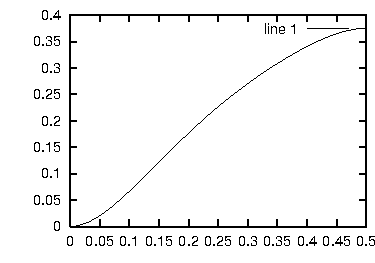
\includegraphics[width=.55\textwidth]{map/pix/learn5.pdf}
        \end{center}
      \end{exparts}
    \end{answer}
  \item 
     Sebuah kota tertentu berada di suatu negara tertentu
     (ini merupakan persoalan hipotetis).
     Setiap tahun, sepuluh persen penduduk kota pindah ke bagian lain negara
     tersebut. Setiap tahun, satu persen orang dari tempat lain pindah ke kota.
     Andaikan terdapat dua keadaan: $s_T$, tinggal di kota, dan $s_C$, tinggal
     di tempat lain.
     \begin{exparts}
       \partsitem Susun matriks transisinya.
       \partsitem Dengan distribusi awal $s_T=0.3$ dan $s_C=0.7$, peroleh
         hasil untuk sepuluh tahun pertama.
       \partsitem Lakukan hal yang sama untuk $s_T=0.2$.
       \partsitem Apakah kedua hasilnya serupa atau berbeda?
     \end{exparts}
     \begin{answer}
       \begin{exparts}
         \partsitem Dari persamaan-persamaan berikut,
           \begin{equation*}
             \begin{linsys}{2}
               0.90\cdot p_{T}(n)  &+  &0.01\cdot p_{C}(n) &= &p_{T}(n+1)   \\
               0.10\cdot p_{T}(n)  &+  &0.99\cdot p_{C}(n) &= &p_{C}(n+1)   
             \end{linsys}
           \end{equation*}
           kita memperoleh matriks berikut.
           \begin{equation*}
             \begin{pmatrix}
               0.90  &0.01  \\
               0.10  &0.99
             \end{pmatrix}
             \colvec{p_{T}(n) \\ p_{C}(n)}
             =
             \colvec{p_{T}(n+1) \\ p_{C}(n+1)}
           \end{equation*}
         \partsitem Berikut hasil dari Octave.
           \begin{center}
             \begin{tabular}{c|ccccc}
               $n=0$ &1  &2  &3  &4  &5  \\ 
               \hline
               $\begin{array}{c}  0.30000 \\ 0.70000 \end{array}$
               &$\begin{array}{c} 0.27700 \\ 0.72300 \end{array}$
               &$\begin{array}{c}  0.25653 \\ 0.74347 \end{array}$
               &$\begin{array}{c}  0.23831 \\ 0.76169 \end{array}$
               &$\begin{array}{c}  0.22210 \\ 0.77790 \end{array}$
               &$\begin{array}{c}  0.20767 \\ 0.79233 \end{array}$
             \end{tabular}                                     \\[1ex]
             \begin{tabular}{|ccccc}
               6  &7  &8  &9 &10 \\ 
               \hline
               $\begin{array}{c}  0.19482 \\ 0.80518 \end{array}$
               &$\begin{array}{c}  0.18339 \\ 0.81661 \end{array}$
               &$\begin{array}{c}  0.17322 \\ 0.82678 \end{array}$
               &$\begin{array}{c}  0.16417 \\ 0.83583 \end{array}$
               &$\begin{array}{c}  0.15611 \\ 0.84389 \end{array}$
             \end{tabular}
           \end{center}
         \partsitem Berikut hasil untuk $s_T=0.2$.
           \begin{center}
             \begin{tabular}{c|ccccc}
               $n=0$ &1  &2  &3  &4  &5  \\ 
               \hline
               $\begin{array}{c}  0.20000 \\ 0.80000 \end{array}$
               &$\begin{array}{c}   0.18800 \\ 0.81200 \end{array}$
               &$\begin{array}{c}   0.17732 \\ 0.82268 \end{array}$
               &$\begin{array}{c}   0.16781 \\ 0.83219 \end{array}$
               &$\begin{array}{c}   0.15936 \\ 0.84064 \end{array}$
               &$\begin{array}{c}   0.15183 \\ 0.84817 \end{array}$
             \end{tabular}                                         \\[1ex]
             \begin{tabular}{|ccccc}
               6  &7  &8  &9 &10 \\ 
               \hline
               $\begin{array}{c}  0.14513 \\ 0.85487  \end{array}$
               &$\begin{array}{c}  0.13916 \\ 0.86084  \end{array}$
               &$\begin{array}{c}  0.13385 \\ 0.86615  \end{array}$
               &$\begin{array}{c}  0.12913 \\ 0.87087  \end{array}$
               &$\begin{array}{c}  0.12493 \\ 0.87507  \end{array}$
             \end{tabular}
           \end{center}
          \partsitem Meskipun vektor probabilitas berawal dengan selisih $0.1$,
            pada akhirnya selisihnya hanya $0.032$.
            Jadi, keduanya serupa.
       \end{exparts}
     \end{answer}  
  \item 
    Untuk penerapan Seri Dunia, gunakan komputer untuk menghasilkan tujuh
    vektor bagi $p=0.55$ dan $p=0.6$.
    \begin{exparts}
      \partsitem Berapakah peluang tim Liga Nasional memenangi seluruh seri,
        meskipun probabilitasnya untuk memenangi satu pertandingan hanya
        $0.45$ atau $0.40$?
      \partsitem Gambarkan grafik probabilitas $p$ terhadap peluang tim Liga
        Amerika memenangi seluruh seri.
        Apakah terdapat nilai ambang\Dash suatu $p$ yang setelahnya tim yang
        lebih kuat pada dasarnya dipastikan menang?
    \end{exparts}
    % (Some sample code is included below.)
    \begin{answer}
     Berikut vektor-vektor untuk $p=.55$ dan $p=0.60$.
     \begin{center}\footnotesize
       \begin{tabular}{@{}r@{}cccccccc@{}}
         &$n=0$  &$n=1$  &$n=2$  &$n=3$  &$n=4$  &$n=5$  &$n=6$  &$n=7$  \\ 
        \hline
        \begin{tabular}{@{}c@{}}
           0-0 \\
           1-0 \\
           0-1 \\
           2-0 \\
           1-1 \\
           0-2 \\
           3-0 \\
           2-1 \\
           1-2 \\
           0-3 \\
           4-0 \\
           3-1 \\
           2-2 \\
           1-3 \\
           0-4 \\
           4-1 \\
           3-2 \\
           2-3 \\
           1-4 \\
           4-2 \\
           3-3 \\
           2-4 \\
           4-3 \\
           3-4
         \end{tabular}
          &$\begin{aligncolondecimal}{0}
             1 \\
             0 \\
             0 \\
             0 \\
             0 \\
             0 \\
             0 \\
             0 \\
             0 \\
             0 \\
             0 \\
             0 \\
             0 \\
             0 \\
             0 \\
             0 \\
             0 \\
             0 \\
             0 \\
             0 \\
             0 \\
             0 \\
             0 \\
             0 
           \end{aligncolondecimal}$     
         &$\begin{aligncolondecimal}{5}
           0 \\
           0.55000 \\
           0.45000 \\
           0 \\
           0 \\
           0 \\
           0 \\
           0 \\
           0 \\
           0 \\
           0 \\
           0 \\
           0 \\
           0 \\
           0 \\
           0 \\
           0 \\
           0 \\
           0 \\
           0 \\
           0 \\
           0 \\
           0 \\
           0
         \end{aligncolondecimal}$
         &$\begin{aligncolondecimal}{5}
           0 \\
           0 \\
           0 \\
           0.30250 \\
           0.49500 \\
           0.20250 \\
           0 \\
           0 \\
           0 \\
           0 \\
           0 \\
           0 \\
           0 \\
           0 \\
           0 \\
           0 \\
           0 \\
           0 \\
           0 \\
           0 \\
           0 \\
           0 \\
           0 \\
           0
         \end{aligncolondecimal}$
         &$\begin{aligncolondecimal}{5}
           0 \\
           0 \\
           0 \\
           0 \\
           0 \\
           0 \\
           0.16638 \\
           0.40837 \\
           0.33412 \\
           0.09112 \\
           0 \\
           0 \\
           0 \\
           0 \\
           0 \\
           0 \\
           0 \\
           0 \\
           0 \\
           0 \\
           0 \\
           0 \\
           0 \\
           0
         \end{aligncolondecimal}$
         &$\begin{aligncolondecimal}{5}
           0 \\
           0 \\
           0 \\
           0 \\
           0 \\
           0 \\
           0 \\
           0 \\
           0 \\
           0 \\
           0.09151 \\
           0.29948 \\
           0.36754 \\
           0.20047 \\
           0.04101 \\
           0 \\
           0 \\
           0 \\
           0 \\
           0 \\
           0 \\
           0 \\
           0 \\
           0
         \end{aligncolondecimal}$
         &$\begin{aligncolondecimal}{5}
          0 \\
          0 \\
          0 \\
          0 \\
          0 \\
          0 \\
          0 \\
          0 \\
          0 \\
          0 \\
          0.09151 \\
          0 \\
          0 \\
          0 \\
          0.04101 \\
          0.16471 \\
          0.33691 \\
          0.27565 \\
          0.09021 \\
          0 \\
          0 \\
          0 \\
          0 \\
          0
         \end{aligncolondecimal}$
         &$\begin{aligncolondecimal}{5}
          0 \\
          0 \\
          0 \\
          0 \\
          0 \\
          0 \\
          0 \\
          0 \\
          0 \\
          0 \\
          0.09151 \\
          0 \\
          0 \\
          0 \\
          0.04101 \\
          0.16471 \\
          0 \\
          0 \\
          0.09021 \\
          0.18530 \\
          0.30322 \\
          0.12404 \\
          0 \\
          0
         \end{aligncolondecimal}$
         &$\begin{aligncolondecimal}{5}
          0 \\
          0 \\
          0 \\
          0 \\
          0 \\
          0 \\
          0 \\
          0 \\
          0 \\
          0 \\
          0.09151 \\
          0 \\
          0 \\
          0 \\
          0.04101 \\
          0.16471 \\
          0 \\
          0 \\
          0.09021 \\
          0.18530 \\
          0 \\
          0.12404 \\
          0.16677 \\
          0.13645
         \end{aligncolondecimal}$
       \end{tabular}                      \\
       % \end{center}
       % and these are the $p=.60$ vectors.
       % \begin{center}\small
       \begin{tabular}{@{}r@{}cccccccc@{}}
         &$n=0$  &$n=1$  &$n=2$  &$n=3$  &$n=4$  &$n=5$  &$n=6$  &$n=7$  \\ 
        \hline
        \begin{tabular}{@{}c@{}}
           0-0 \\
           1-0 \\
           0-1 \\
           2-0 \\
           1-1 \\
           0-2 \\
           3-0 \\
           2-1 \\
           1-2 \\
           0-3 \\
           4-0 \\
           3-1 \\
           2-2 \\
           1-3 \\
           0-4 \\
           4-1 \\
           3-2 \\
           2-3 \\
           1-4 \\
           4-2 \\
           3-3 \\
           2-4 \\
           4-3 \\
           3-4
         \end{tabular}
          &$\begin{aligncolondecimal}{0}
             1 \\
             0 \\
             0 \\
             0 \\
             0 \\
             0 \\
             0 \\
             0 \\
             0 \\
             0 \\
             0 \\
             0 \\
             0 \\
             0 \\
             0 \\
             0 \\
             0 \\
             0 \\
             0 \\
             0 \\
             0 \\
             0 \\
             0 \\
             0 
           \end{aligncolondecimal}$     
         &$\begin{aligncolondecimal}{5}
          0 \\
          0.60000 \\
          0.40000 \\
          0 \\
          0 \\
          0 \\
          0 \\
          0 \\
          0 \\
          0 \\
          0 \\
          0 \\
          0 \\
          0 \\
          0 \\
          0 \\
          0 \\
          0 \\
          0 \\
          0 \\
          0 \\
          0 \\
          0 \\
          0               
         \end{aligncolondecimal}$
         &$\begin{aligncolondecimal}{5}
            0 \\
            0 \\
            0 \\
            0.36000 \\
            0.48000 \\
            0.16000 \\
            0 \\
            0 \\
            0 \\
            0 \\
            0 \\
            0 \\
            0 \\
            0 \\
            0 \\
            0 \\
            0 \\
            0 \\
            0 \\
            0 \\
            0 \\
            0 \\
            0 \\
            0         
         \end{aligncolondecimal}$
         &$\begin{aligncolondecimal}{5}
            0 \\
            0 \\
            0 \\
            0 \\
            0 \\
            0 \\
            0.21600 \\
            0.43200 \\
            0.28800 \\
            0.06400 \\
            0 \\
            0 \\
            0 \\
            0 \\
            0 \\
            0 \\
            0 \\
            0 \\
            0 \\
            0 \\
            0 \\
            0 \\
            0 \\
            0         
         \end{aligncolondecimal}$
         &$\begin{aligncolondecimal}{5}
            0 \\
            0 \\
            0 \\
            0 \\
            0 \\
            0 \\
            0 \\
            0 \\
            0 \\
            0 \\
            0.12960 \\
            0.34560 \\
            0.34560 \\
            0.15360 \\
            0.02560 \\
            0 \\
            0 \\
            0 \\
            0 \\
            0 \\
            0 \\
            0 \\
            0 \\
            0         
         \end{aligncolondecimal}$
         &$\begin{aligncolondecimal}{5}
             0 \\
             0 \\
             0 \\
             0 \\
             0 \\
             0 \\
             0 \\
             0 \\
             0 \\
             0 \\
             0.12960 \\
             0 \\
             0 \\
             0 \\
             0.02560 \\
             0.20736 \\
             0.34560 \\
             0.23040 \\
             0.06144 \\
             0 \\
             0 \\
             0 \\
             0 \\
             0          
         \end{aligncolondecimal}$
         &$\begin{aligncolondecimal}{5}
            0 \\
            0 \\
            0 \\
            0 \\
            0 \\
            0 \\
            0 \\
            0 \\
            0 \\
            0 \\
            0.12960 \\
            0 \\
            0 \\
            0 \\
            0.02560 \\
            0.20736 \\
            0 \\
            0 \\
            0.06144 \\
            0.20736 \\
            0.27648 \\
            0.09216 \\
            0 \\
            0         
         \end{aligncolondecimal}$
         &$\begin{aligncolondecimal}{5}
            0 \\
            0 \\
            0 \\
            0 \\
            0 \\
            0 \\
            0 \\
            0 \\
            0 \\
            0 \\
            0.12960 \\
            0 \\
            0 \\
            0 \\
            0.02560 \\
            0.20736 \\
            0 \\
            0 \\
            0.06144 \\
            0.20736 \\
            0 \\
            0.09216 \\
            0.16589 \\
            0.11059         
         \end{aligncolondecimal}$
       \end{tabular}
     \end{center}
     \begin{exparts}
      \partsitem Kita dapat mengadaptasi skrip dari bagian akhir Topik ini.
\begin{lstlisting}
# Berkas skrip Octave untuk menghitung peluang hasil Seri Dunia.
function w = markov(p,v)
  q = 1-p;
  A=[0,0,0,0,0,0, 0,0,0,0,0,0, 0,0,0,0,0,0, 0,0,0,0,0,0;  # 0-0
     p,0,0,0,0,0, 0,0,0,0,0,0, 0,0,0,0,0,0, 0,0,0,0,0,0;  # 1-0
     q,0,0,0,0,0, 0,0,0,0,0,0, 0,0,0,0,0,0, 0,0,0,0,0,0;  # 0-1_
     0,p,0,0,0,0, 0,0,0,0,0,0, 0,0,0,0,0,0, 0,0,0,0,0,0;  # 2-0
     0,q,p,0,0,0, 0,0,0,0,0,0, 0,0,0,0,0,0, 0,0,0,0,0,0;  # 1-1
     0,0,q,0,0,0, 0,0,0,0,0,0, 0,0,0,0,0,0, 0,0,0,0,0,0;  # 0-2__
     0,0,0,p,0,0, 0,0,0,0,0,0, 0,0,0,0,0,0, 0,0,0,0,0,0;  # 3-0
     0,0,0,q,p,0, 0,0,0,0,0,0, 0,0,0,0,0,0, 0,0,0,0,0,0;  # 2-1
     0,0,0,0,q,p, 0,0,0,0,0,0, 0,0,0,0,0,0, 0,0,0,0,0,0;  # 1-2_
     0,0,0,0,0,q, 0,0,0,0,0,0, 0,0,0,0,0,0, 0,0,0,0,0,0;  # 0-3
     0,0,0,0,0,0, p,0,0,0,1,0, 0,0,0,0,0,0, 0,0,0,0,0,0;  # 4-0
     0,0,0,0,0,0, q,p,0,0,0,0, 0,0,0,0,0,0, 0,0,0,0,0,0;  # 3-1__
     0,0,0,0,0,0, 0,q,p,0,0,0, 0,0,0,0,0,0, 0,0,0,0,0,0;  # 2-2
     0,0,0,0,0,0, 0,0,q,p,0,0, 0,0,0,0,0,0, 0,0,0,0,0,0;  # 1-3
     0,0,0,0,0,0, 0,0,0,q,0,0, 0,0,1,0,0,0, 0,0,0,0,0,0;  # 0-4_
     0,0,0,0,0,0, 0,0,0,0,0,p, 0,0,0,1,0,0, 0,0,0,0,0,0;  # 4-1
     0,0,0,0,0,0, 0,0,0,0,0,q, p,0,0,0,0,0, 0,0,0,0,0,0;  # 3-2
     0,0,0,0,0,0, 0,0,0,0,0,0, q,p,0,0,0,0, 0,0,0,0,0,0;  # 2-3__
     0,0,0,0,0,0, 0,0,0,0,0,0, 0,q,0,0,0,0, 1,0,0,0,0,0;  # 1-4
     0,0,0,0,0,0, 0,0,0,0,0,0, 0,0,0,0,p,0, 0,1,0,0,0,0;  # 4-2
     0,0,0,0,0,0, 0,0,0,0,0,0, 0,0,0,0,q,p, 0,0,0,0,0,0;  # 3-3_
     0,0,0,0,0,0, 0,0,0,0,0,0, 0,0,0,0,0,q, 0,0,0,1,0,0;  # 2-4
     0,0,0,0,0,0, 0,0,0,0,0,0, 0,0,0,0,0,0, 0,0,p,0,1,0;  # 4-3
     0,0,0,0,0,0, 0,0,0,0,0,0, 0,0,0,0,0,0, 0,0,q,0,0,1]; # 3-4
  v7 = (A**7) * v;
  w = v7(11)+v7(16)+v7(20)+v7(23)
endfunction
\end{lstlisting}
       Ketika tim Liga Amerika memiliki probabilitas $p=0.55$ untuk memenangi
       setiap pertandingan, probabilitasnya untuk memenangi seri adalah
       $0.60829$, sehingga probabilitas tim Liga Nasional adalah $0.39171$.
       Ketika probabilitas Liga Amerika untuk memenangi satu pertandingan
       adalah $p=0.6$, probabilitasnya untuk memenangi seri adalah $0.71021$,
       sehingga probabilitas Liga Nasional adalah $0.28979$.
      \partsitem Dari sesi Octave dan grafik berikut,
\begin{lstlisting}
octave:1> v0=[1;0;0;0;0;0;0;0;0;0;0;0;0;0;0;0;0;0;0;0;0;0;0;0];
octave:2> x=(.01:.01:.99)';
octave:3> y=(.01:.01:.99)';
octave:4> for i=.01:.01:.99
>          y(100*i)=markov(i,v0);
>         endfor
octave:5> z=[x, y];
octave:6> gplot z
\end{lstlisting}
       secara visual kita menilai bahwa jika $p>0.7$, tim tersebut hampir
       dipastikan memenangi seri.
       \begin{center}
         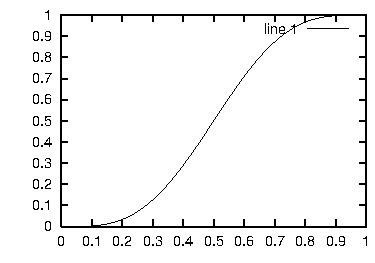
\includegraphics[width=0.4\textwidth]{map/pix/ws.pdf}
       \end{center}
     \end{exparts}
    \end{answer}
  \item 
    Di atas, kita mendefinisikan matriks transisi sebagai matriks yang setiap
    entrinya tak negatif dan setiap kolomnya berjumlah $1$.
    \begin{exparts}
      \partsitem Periksa bahwa ketiga matriks transisi yang ditampilkan dalam Topik
        ini memenuhi kedua syarat tersebut.
        Haruskah setiap matriks transisi memenuhinya?
      \partsitem Perhatikan bahwa jika $A\vec{v}_0=\vec{v}_1$ dan
        $A\vec{v}_1=\vec{v}_2$, maka $A^2$ merupakan matriks transisi dari
        $\vec{v}_0$ ke $\vec{v}_2$.
        Tunjukkan bahwa pangkat suatu matriks transisi juga merupakan matriks
        transisi.
      \partsitem Perumum butir sebelumnya dengan membuktikan bahwa hasil kali dua
        matriks transisi yang ukurannya sesuai merupakan matriks transisi.
    \end{exparts}
    \begin{answer}
      \begin{exparts}
        \partsitem Matriks-matriks itu harus memenuhi kedua syarat tersebut:
          setiap entri merupakan probabilitas sehingga tak negatif, dan
          probabilitas total transisi dari suatu keadaan (termasuk kembali ke
          keadaan yang sama) adalah $100\%$.
        \partsitem Lihat jawaban untuk butir ketiga.
        \partsitem Kita akan mengerjakan kasus $\nbyn{2}$; kasus berukuran
          lebih besar hanya menimbulkan persoalan notasi.
          Setiap entri hasil kali tak negatif karena merupakan jumlah hasil
          kali bilangan-bilangan tak negatif.
          Hasil kali berikut
          \begin{equation*}
            \begin{pmatrix}
              a_{1,1}  &a_{1,2}  \\
              a_{2,1}  &a_{2,2}  
            \end{pmatrix}
            \begin{pmatrix}
              b_{1,1}  &b_{1,2}  \\
              b_{2,1}  &b_{2,2}  
            \end{pmatrix}
            =\begin{pmatrix}
              a_{1,1}b_{1,1}+a_{1,2}b_{2,1}  &a_{1,1}b_{1,2}+a_{1,2}b_{2,2} \\
              a_{2,1}b_{1,1}+a_{2,2}b_{2,1}  &a_{2,1}b_{1,2}+a_{2,2}b_{2,2} \\
            \end{pmatrix}
           \end{equation*}
             memiliki dua jumlah kolom berikut,
            \begin{multline*}
              (a_{1,1}b_{1,1}+a_{1,2}b_{2,1})
              +(a_{2,1}b_{1,1}+a_{2,2}b_{2,1})
              =(a_{1,1}+a_{2,1})\cdot b_{1,1}
                +(a_{1,2}+a_{2,2})\cdot b_{2,1}            \\
              =1\cdot b_{1,1}+1\cdot b_{2,1}
              =1
            \end{multline*}
             dan
            \begin{multline*}
              (a_{1,1}b_{1,2}+a_{1,2}b_{2,2})
              +(a_{2,1}b_{1,2}+a_{2,2}b_{2,2})
              =(a_{1,1}+a_{2,1})\cdot b_{1,2}
                +(a_{1,2}+a_{2,2})\cdot b_{2,2}              \\
              =1\cdot b_{1,2}+1\cdot b_{2,2}
              =1
            \end{multline*}
             seperti yang diperlukan.
      \end{exparts}
    \end{answer}
\end{exercises}


% \announcecomputercode
% This script \textit{markov.m} for the computer algebra system Octave 
% generated the table of World Series outcomes.
% (The hash character \texttt{\#} marks the rest of a line as a comment.)
% \begin{lstlisting}
% # Octave script file to compute chance of World Series outcomes.
% function w = markov(p,v)
%   q = 1-p;
%   A=[0,0,0,0,0,0, 0,0,0,0,0,0, 0,0,0,0,0,0, 0,0,0,0,0,0;  # 0-0
%      p,0,0,0,0,0, 0,0,0,0,0,0, 0,0,0,0,0,0, 0,0,0,0,0,0;  # 1-0
%      q,0,0,0,0,0, 0,0,0,0,0,0, 0,0,0,0,0,0, 0,0,0,0,0,0;  # 0-1_
%      0,p,0,0,0,0, 0,0,0,0,0,0, 0,0,0,0,0,0, 0,0,0,0,0,0;  # 2-0
%      0,q,p,0,0,0, 0,0,0,0,0,0, 0,0,0,0,0,0, 0,0,0,0,0,0;  # 1-1
%      0,0,q,0,0,0, 0,0,0,0,0,0, 0,0,0,0,0,0, 0,0,0,0,0,0;  # 0-2__
%      0,0,0,p,0,0, 0,0,0,0,0,0, 0,0,0,0,0,0, 0,0,0,0,0,0;  # 3-0
%      0,0,0,q,p,0, 0,0,0,0,0,0, 0,0,0,0,0,0, 0,0,0,0,0,0;  # 2-1
%      0,0,0,0,q,p, 0,0,0,0,0,0, 0,0,0,0,0,0, 0,0,0,0,0,0;  # 1-2_
%      0,0,0,0,0,q, 0,0,0,0,0,0, 0,0,0,0,0,0, 0,0,0,0,0,0;  # 0-3
%      0,0,0,0,0,0, p,0,0,0,1,0, 0,0,0,0,0,0, 0,0,0,0,0,0;  # 4-0
%      0,0,0,0,0,0, q,p,0,0,0,0, 0,0,0,0,0,0, 0,0,0,0,0,0;  # 3-1__
%      0,0,0,0,0,0, 0,q,p,0,0,0, 0,0,0,0,0,0, 0,0,0,0,0,0;  # 2-2
%      0,0,0,0,0,0, 0,0,q,p,0,0, 0,0,0,0,0,0, 0,0,0,0,0,0;  # 1-3
%      0,0,0,0,0,0, 0,0,0,q,0,0, 0,0,1,0,0,0, 0,0,0,0,0,0;  # 0-4_
%      0,0,0,0,0,0, 0,0,0,0,0,p, 0,0,0,1,0,0, 0,0,0,0,0,0;  # 4-1
%      0,0,0,0,0,0, 0,0,0,0,0,q, p,0,0,0,0,0, 0,0,0,0,0,0;  # 3-2
%      0,0,0,0,0,0, 0,0,0,0,0,0, q,p,0,0,0,0, 0,0,0,0,0,0;  # 2-3__
%      0,0,0,0,0,0, 0,0,0,0,0,0, 0,q,0,0,0,0, 1,0,0,0,0,0;  # 1-4
%      0,0,0,0,0,0, 0,0,0,0,0,0, 0,0,0,0,p,0, 0,1,0,0,0,0;  # 4-2
%      0,0,0,0,0,0, 0,0,0,0,0,0, 0,0,0,0,q,p, 0,0,0,0,0,0;  # 3-3_
%      0,0,0,0,0,0, 0,0,0,0,0,0, 0,0,0,0,0,q, 0,0,0,1,0,0;  # 2-4
%      0,0,0,0,0,0, 0,0,0,0,0,0, 0,0,0,0,0,0, 0,0,p,0,1,0;  # 4-3
%      0,0,0,0,0,0, 0,0,0,0,0,0, 0,0,0,0,0,0, 0,0,q,0,0,1]; # 3-4
%   w = A * v;
% endfunction
% \end{lstlisting}
% \noindent Then the Octave session was this.
% \begin{lstlisting}
% > v0=[1;0;0;0;0;0;0;0;0;0;0;0;0;0;0;0;0;0;0;0;0;0;0;0]
% > p=.5
% > v1=markov(p,v0)
% > v2=markov(p,v1)
%   ...
% \end{lstlisting}
% \noindent Translating to another computer algebra system should be 
% easy\Dash all 
% have commands similar to these.
\index{rantai Markov|)}
\endinput
